\documentclass[aspectratio=169]{beamer}

% Theme
\usetheme{metropolis}
\metroset{numbering=fraction,progressbar=frametitle}

% Minimal, safe packages
\usepackage{amsmath,amssymb}
\usepackage{booktabs}
\usepackage{graphicx}
\usepackage{hyperref}

% (Optional) bullet shapes for clarity
\setbeamertemplate{itemize items}[circle]
\setbeamertemplate{itemize subitem}[triangle]

% Metadata
\title{Write-up for Allan}
\date{\today}

\begin{document}

% Title


% Title
\frame{\titlepage}

% Slide 1
\begin{frame}{Descriptives I Want to Present}
\begin{itemize}
  \item Substitution patterns for buildings.
  \item Price changes post-COVID.
  \item Eviction changes post-COVID.
  \item Landlord responses to changes in tenant protections:
    \begin{itemize}
      \item Price changes.
      \item Exit.
      \item Changes in filing behavior.
    \end{itemize}
  \item GE / spillover effects:
    \begin{itemize}
      \item Changes in neighborhood prices.
    \end{itemize}
\end{itemize}
\end{frame}


% Slide 2
\begin{frame}{Substitution Patterns for Buildings}
InfoUSA address flows between buildings; examine whether people in high-evicting buildings are more likely to move to high-evicting buildings.
\begin{itemize}
  \item Not sure of the best way to do this.
  \item Things I have tried: gravity equation.
\end{itemize}

\medskip
\textbf{Equation idea:}
\begin{align}
\operatorname{filing\_rate}_{d}
  &= \beta_0 
   + \beta_1\,\operatorname{filing\_rate}_{o}
   + \boldsymbol{\beta}_2^{\top} \mathbf{X}^{\text{origin}}_{o}
   + \boldsymbol{\beta}_3^{\top} \mathbf{X}^{\text{dest}}_{d}
   + \gamma_{n(o)} + \delta_{n(d)} + \varepsilon_{od}
   \label{eq:filing-rate-flows}
\end{align}

{\small where \(o\) = origin property, \(d\) = destination property, and \(n(\cdot)\) indexes neighborhood fixed effects.}

\medskip
Very significant \(\beta_1\) and high partial \(R^2\).
\end{frame}

% Slide 3
\begin{frame}{Post-COVID Pricing}
Following that one labor paper, the best approach is a series of price indices:
\begin{itemize}
  \item One for the broader rental market.
  \item One for the broader low-income rental market.
  \item One for the high-evicting market.
\end{itemize}

When I estimate event-study coefficients with “treatment” defined as post-COVID, I obtain large relative price increases for high-evicting buildings, although the timing is somewhat tricky.
\end{frame}


\begin{frame}{Post-COVID Pricing: Results}
\begin{figure}
  \includegraphics[width=\linewidth]{}
  \fbox{\rule{0pt}{2.2in}\rule{0.95\linewidth}{0pt}}
\end{figure}
\end{frame}


\begin{frame}{Descriptives on Changes in Eviction Filing Rates}
I want to show that there has been a meaningful change in aggregate filing rates. Then, given these changes, I want to ask what kinds of landlords/properties are changing their filing rates.
\end{frame}


% Slide 4
\begin{frame}{Aggregate Eviction Changes to Tenant Protections}
Big aggregate drops.

\medskip
\begin{figure}
  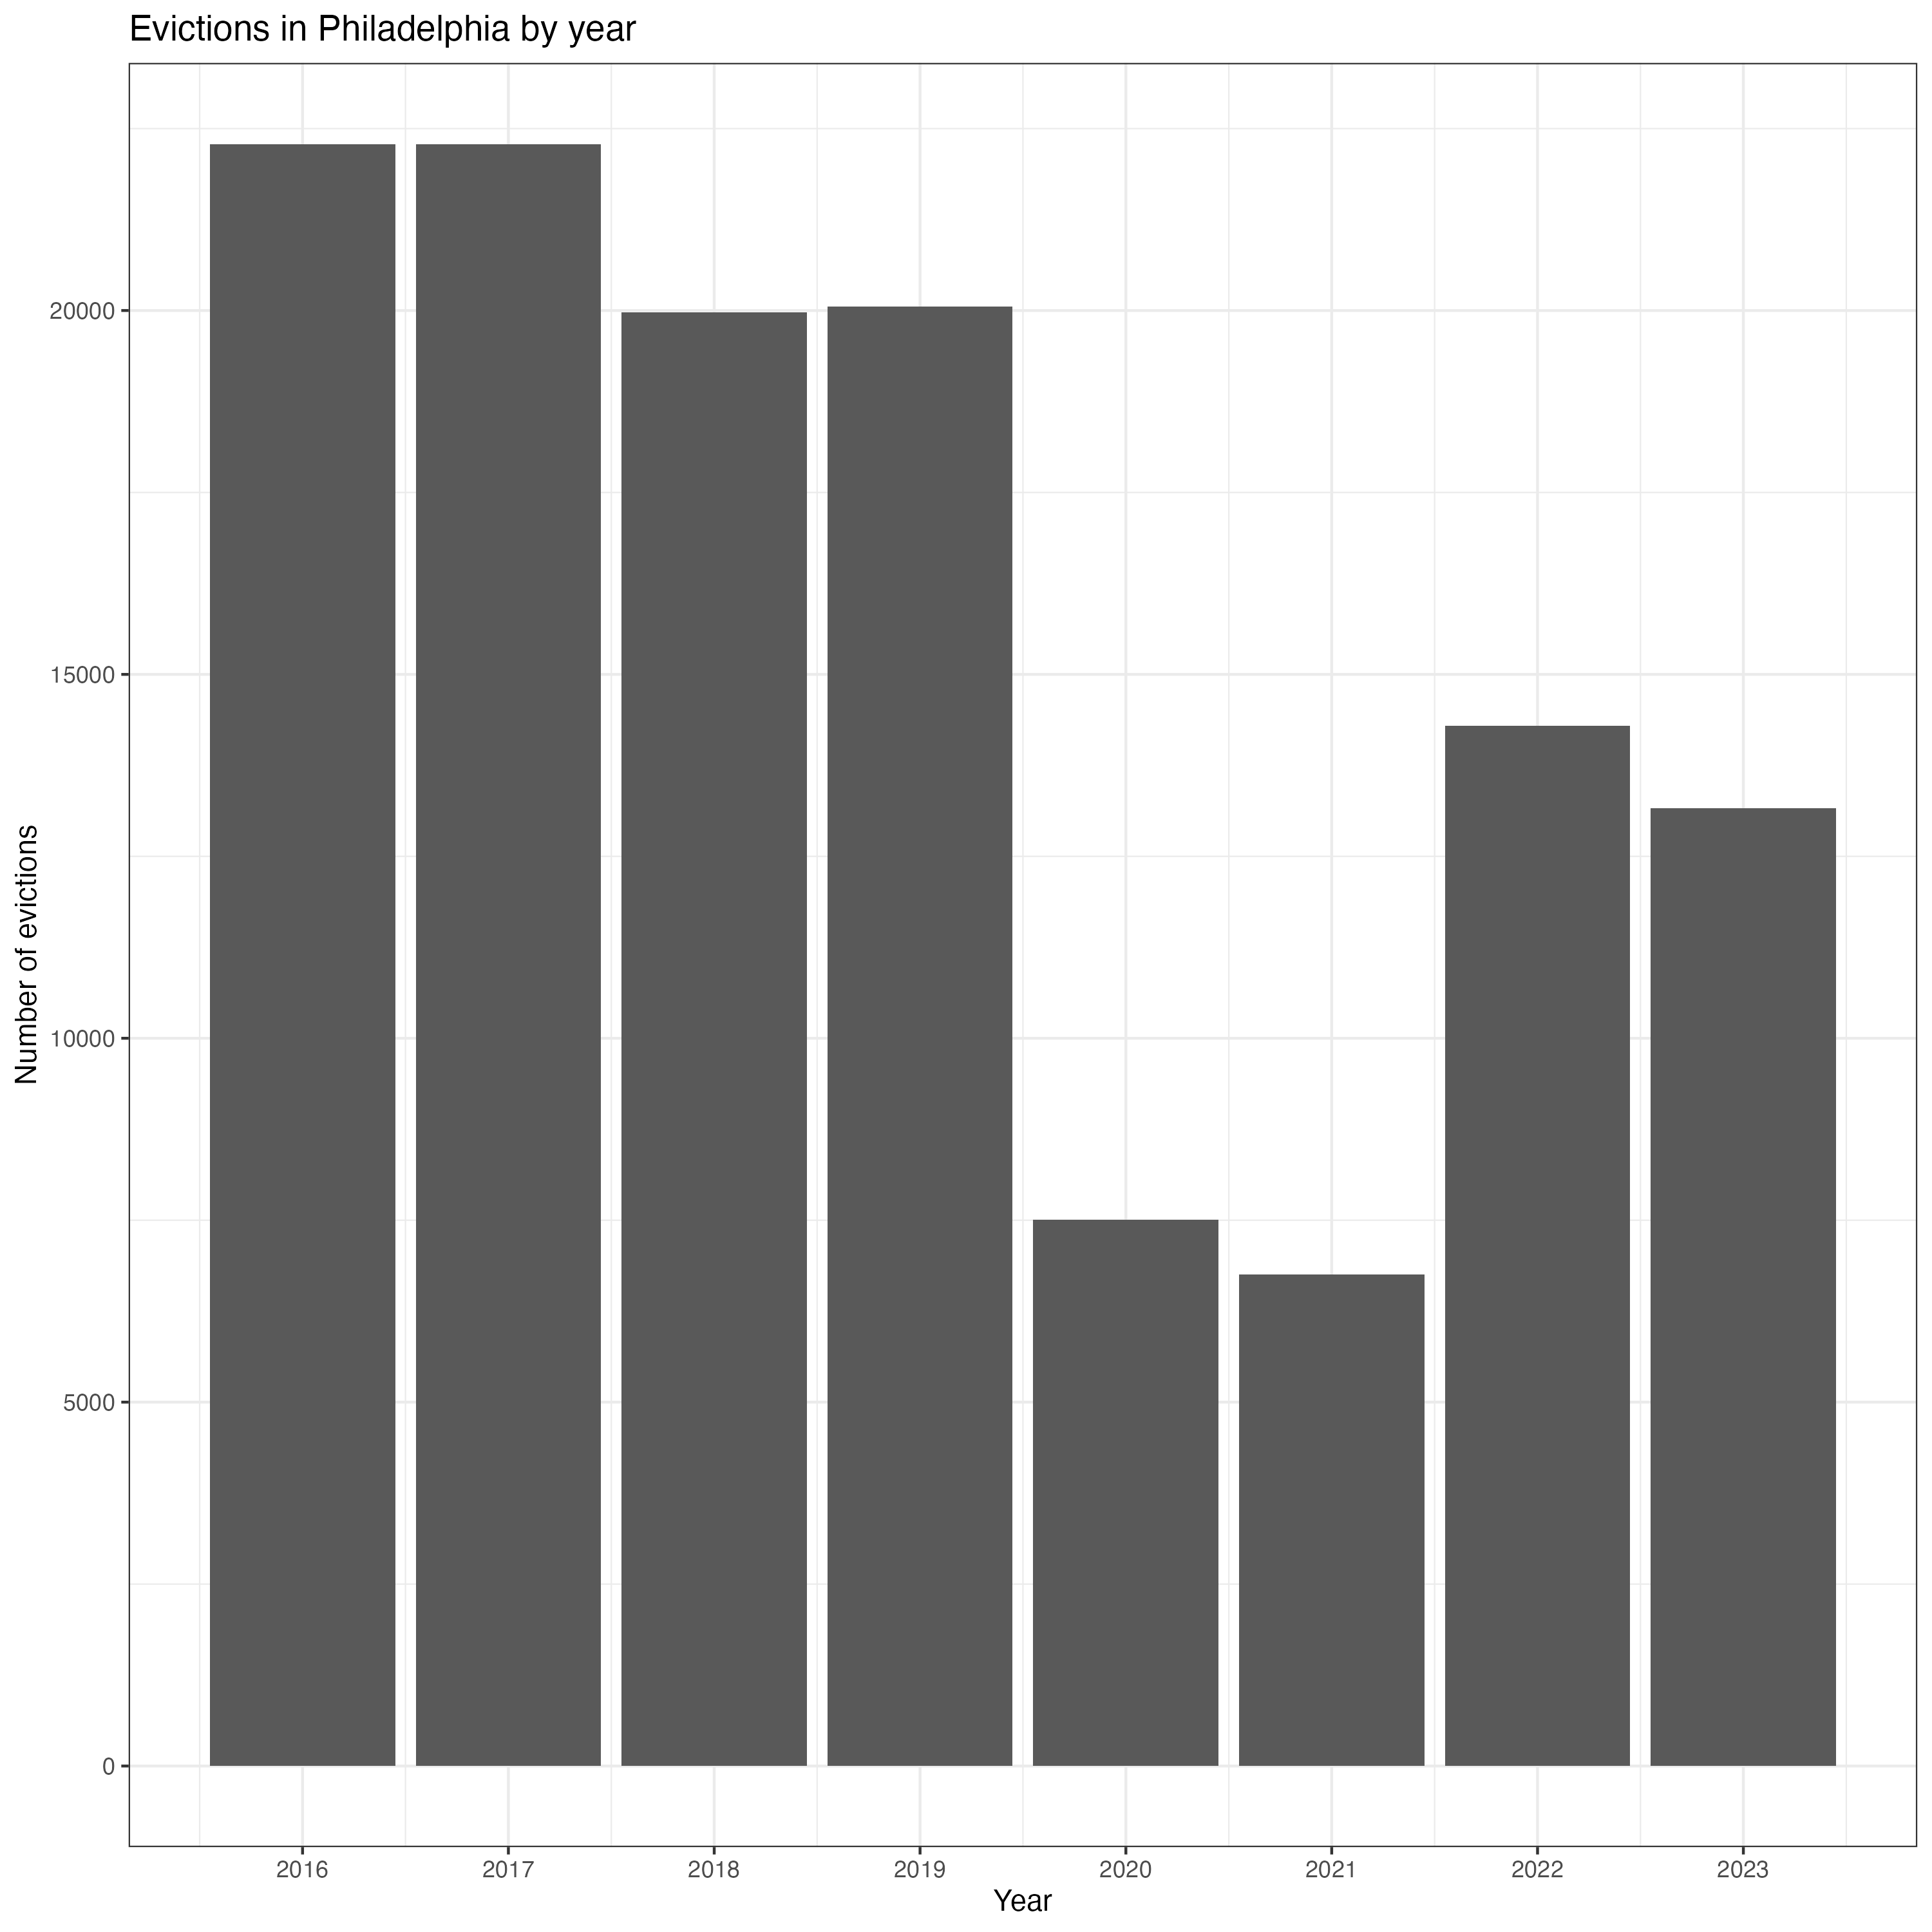
\includegraphics[width=\linewidth]{figs/evict_by_year.png}
  \fbox{\rule{0pt}{2.2in}\rule{0.95\linewidth}{0pt}}
\end{figure}
\end{frame}


% Slide 5
\begin{frame}{Building Changes to Tenant Protections}
Largest drops by landlords who had the highest pre-filing rates.

\medskip
\begin{figure}
  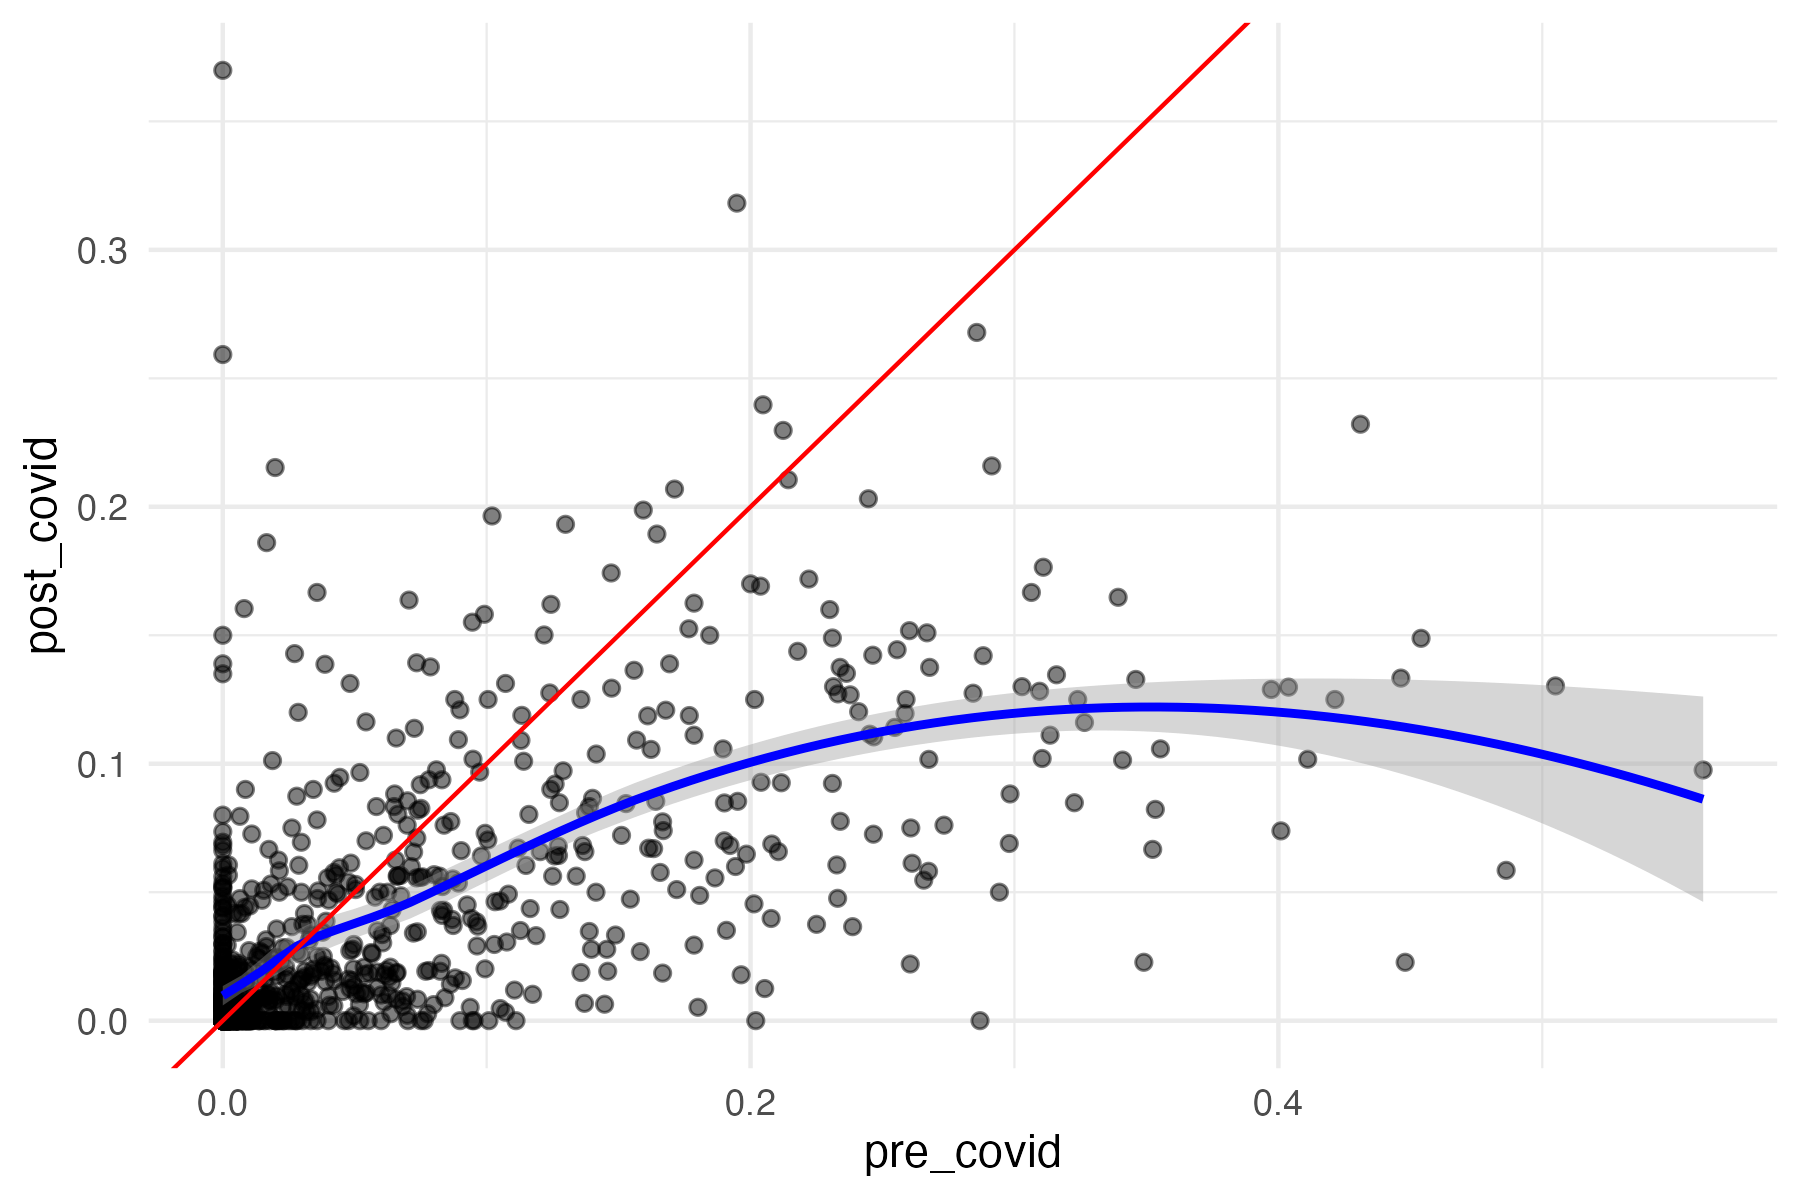
\includegraphics[width=\linewidth]{figs/filing_rate_pre_post_covid.png}
  \fbox{\rule{0pt}{2.2in}\rule{0.95\linewidth}{0pt}}
\end{figure}

\begin{itemize}
  \item You would expect some of this from mean reversion.
\end{itemize}
\end{frame}


% Slide 6
\begin{frame}{Landlord Exit}
Want to identify marginal/inframarginal landlord.\\
Key will be that optimal regulation targets high-evicting landlords with poor outside options.

\medskip
\begin{itemize}
  \item Building sales (doable).
  \item Exit from rental registry (doable).
  \item Condo conversion (doable).
  \item AirBnB (doable, but requires data purchase).
\end{itemize}
\end{frame}


% Slide 7
\begin{frame}{GE / Spillover Effects}
\begin{itemize}
  \item Rental prices by neighborhood.
  \item Rental prices for close substitutes for high-evicting buildings.
\end{itemize}
\end{frame}


% Slide 8
\begin{frame}{Slumlord Model}
Key economics will be that optimal regulation involves targeting landlords with high filing rates that have poor outside options
\begin{itemize}
  \item Get exit thresholds (scrap value?) for different kinds of landlords.
  \item Given exit thresholds, do policy counterfactuals with different changes in filing rates
\end{itemize}
\end{frame}


% Slide 9 (Appendix)
\appendix

\begin{frame}{Appendix of Other Things}
Right now, the only case study is Philly, but if I don't mind having worse rental data, I can add in other cities that have changed eviction policies
    
\end{frame}

\begin{frame}{Appendix of Misc Issues}
How to think about single-family homes?
\begin{itemize}
  \item Philadelphia has a large number of single-family rentals.
  \item Not professionally managed; big source of affordability.
  \item An SFR would be “high-evicting” if it had one eviction in ten years; this is odd to interpret.
\end{itemize}
\end{frame}

\end{document}


\end{document}
